\begin{frame}{Evaluation: Generated Profiles}
  \begin{figure}
    \centering
    \begin{subfigure}[t]{0.48\textwidth}
      \centering
      \caption{Augmented Reality (AR)}
      \label{fig:ar-profile}
      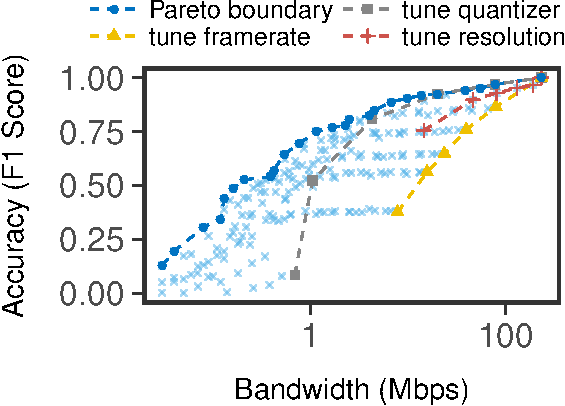
\includegraphics[width=\textwidth]{figures/profile-darknet.pdf}
    \end{subfigure}
    \hfill
    \begin{subfigure}[t]{0.48\textwidth}
      \centering
      \caption{Pedestrian Detection (PD)}
      \label{fig:pd-profile}
      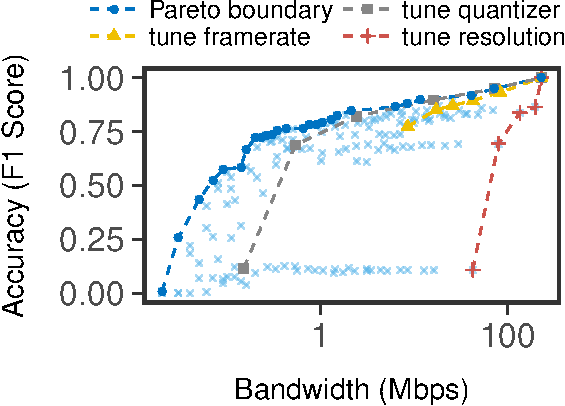
\includegraphics[width=\textwidth]{figures/profile-mot.pdf}
    \end{subfigure}
  \end{figure}

  \begin{itemize}
    \footnotesize
    \visible<2->{
    \item Optimal strategy is achieved with multiple dimensions; tuning one
      dimension leads to suboptimal performance.
    }
    \visible<3->{
    \item For the same application, different dimensions have different impact.
    }
    \visible<4->{\item For different applications, the same dimension has different
      impact.
    }
  \end{itemize}
\end{frame}

\begin{frame}{Evaluation: Generated Profiles (Top-K)}
  \begin{columns}
    \begin{column}{0.45\textwidth}
      \begin{figure}
        \centering
        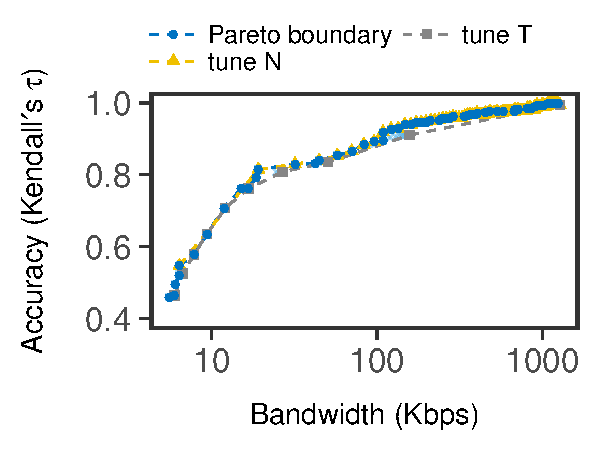
\includegraphics[width=\textwidth]{figures/profile-topk.pdf}
      \end{figure}
    \end{column}
    \begin{column}{0.55\textwidth}
      \begin{itemize}
        \visible<2->{
        \item The effect of each dimension is not significantly different.
        }
        \visible<3->{
        \item The profile offers quantified effects of degradation.
        }
      \end{itemize}
    \end{column}
  \end{columns}
\end{frame}

\begin{frame}{Evaluation: Runtime Experiment Baselines}
  \vspace{1em}
  \only<1-4>{
  \begin{table}
    \footnotesize
    \centering
    \begin{tabular}{ c m{0.6\linewidth} }
      \toprule
      \textbf{Baseline} & \textbf{Description} \\
      \midrule
      Streaming over TCP & A non-adaptive approach \\
      \midrule
      Streaming over UDP & A non-adaptive approach, represents RTP/UDP/RTSP
                           video streaming \\
      \midrule
      \visible<2->{
      \specialcell{JetStream\\\cite{rabkin2014aggregation}}
                        & Manual Policy: \textit{``if bandwidth is insufficient, switch to
                          sending images at 75\% fidelity, then 50\% if there still isn't enough
                          bandwidth. Beyond that point, reduce the frame rate, but keep the image
                          fidelity.''} \\
      \midrule
      }
      \visible<3->{
      JetStream++ & Uses adaptation policy generated by AWStream. JetStream
                    runtime does not probe (hence may oscillate between policies). \\
      \midrule
      }
      \visible<4->{
      \specialcell{HLS\\\cite{pantos2016http}}
                        & HTTP Live Streaming represents popular adaptive video
                          streaming techniques; used for Periscope video stream~\cite{wang2016anatomy}. \\
      \bottomrule
      }
    \end{tabular}
  \end{table}
  }

  \only<5->{
    \begin{figure}
      \centering
      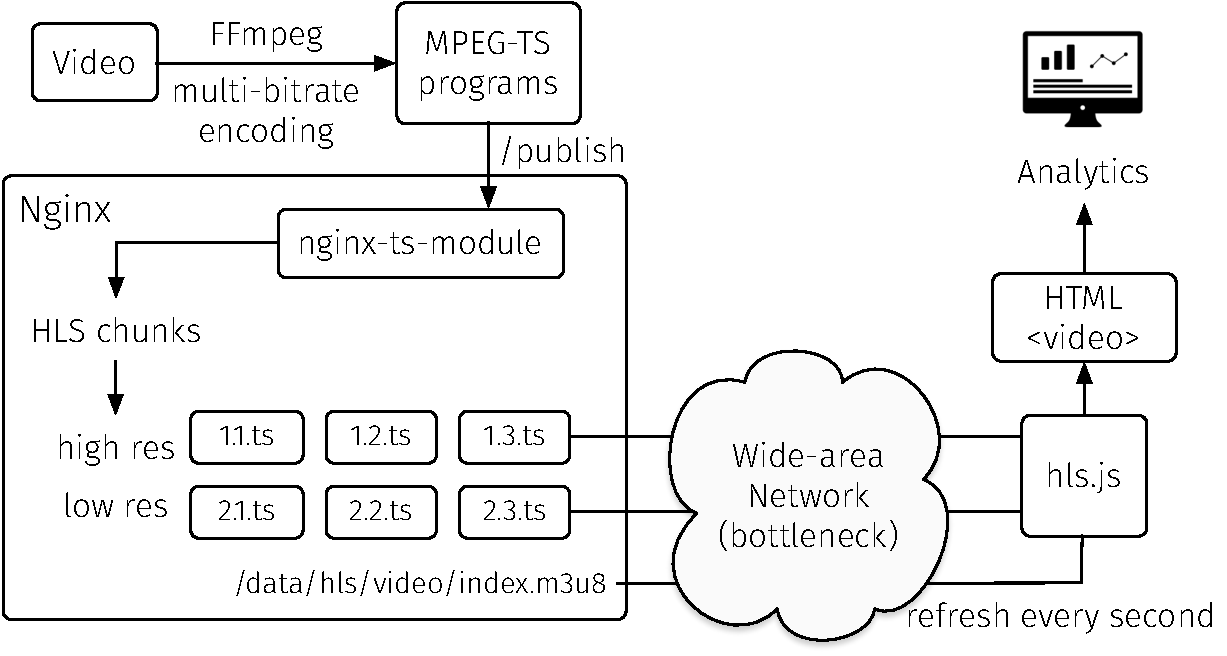
\includegraphics[width=0.8\textwidth]{figures/hls.pdf}
      \caption{HTTP Live Streaming (HLS) architecture: designed for live video
        viewing and relying on buffering at the viewing side.}
    \end{figure}
  }
\end{frame}

\begin{frame}{Evaluation: Runtime Performance}
  \only<1-5>{
    \begin{figure}
      \centering
      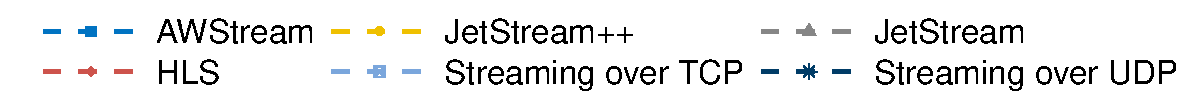
\includegraphics[width=0.8\textwidth]{figures/runtime-timeseries-legend.pdf}
    \end{figure}
    \vspace{-1em}
  }
  \only<1>{
    \begin{figure}
      \centering
      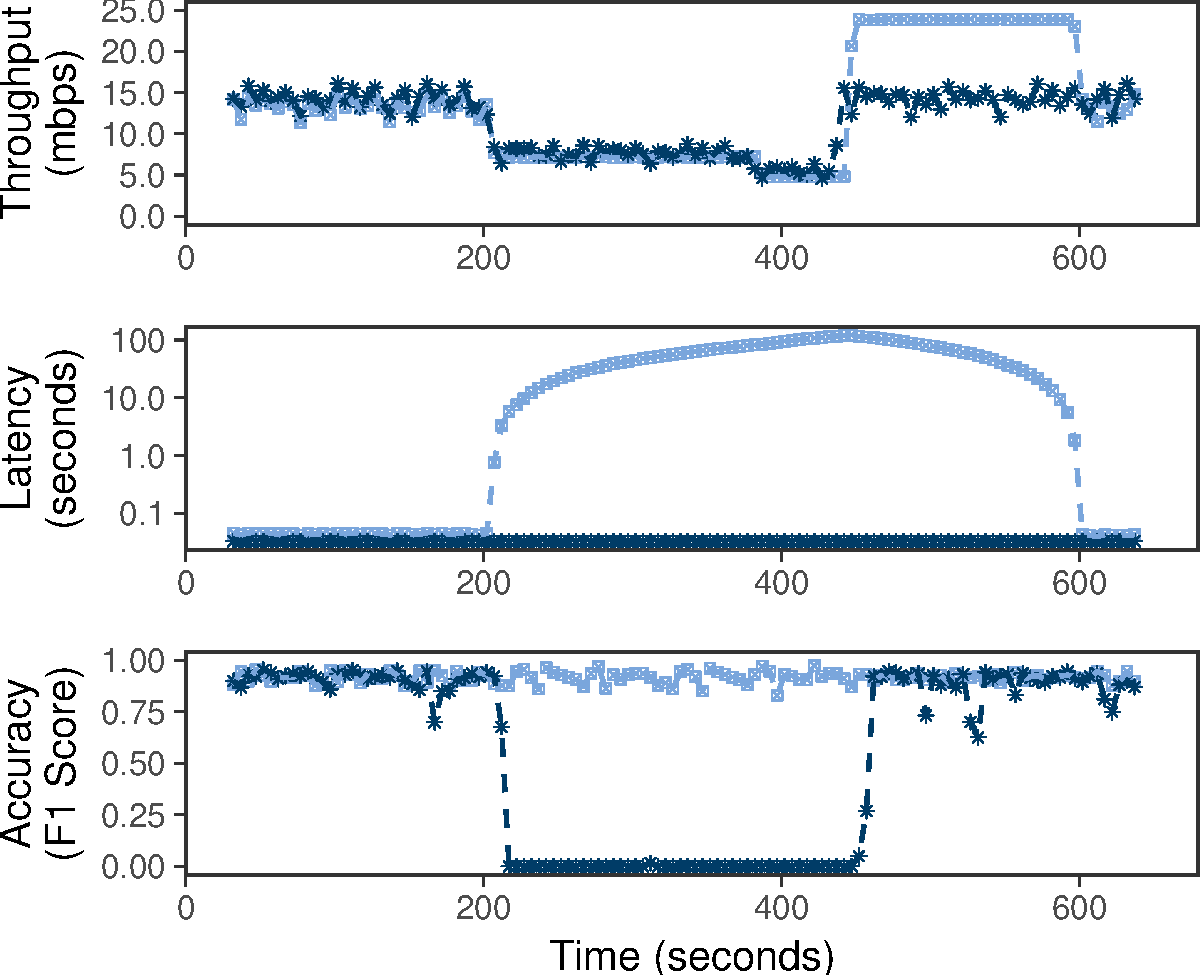
\includegraphics[width=0.8\textwidth]{figures/runtime-timeseries-1.pdf}
    \end{figure}
  }
  \only<2>{
    \begin{figure}
      \centering
      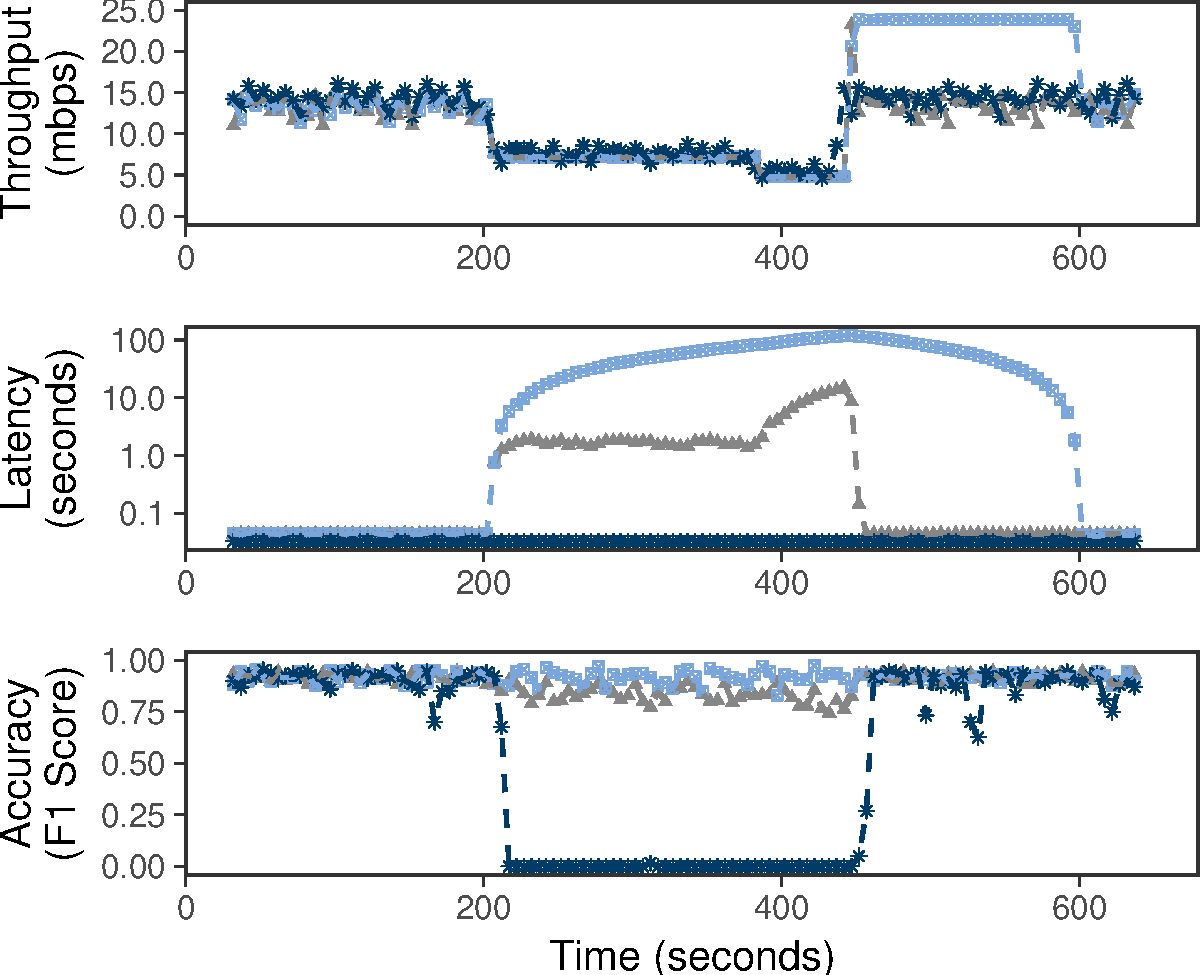
\includegraphics[width=0.8\textwidth]{figures/runtime-timeseries-2.pdf}
    \end{figure}
  }
  \only<3>{
    \begin{figure}
      \centering
      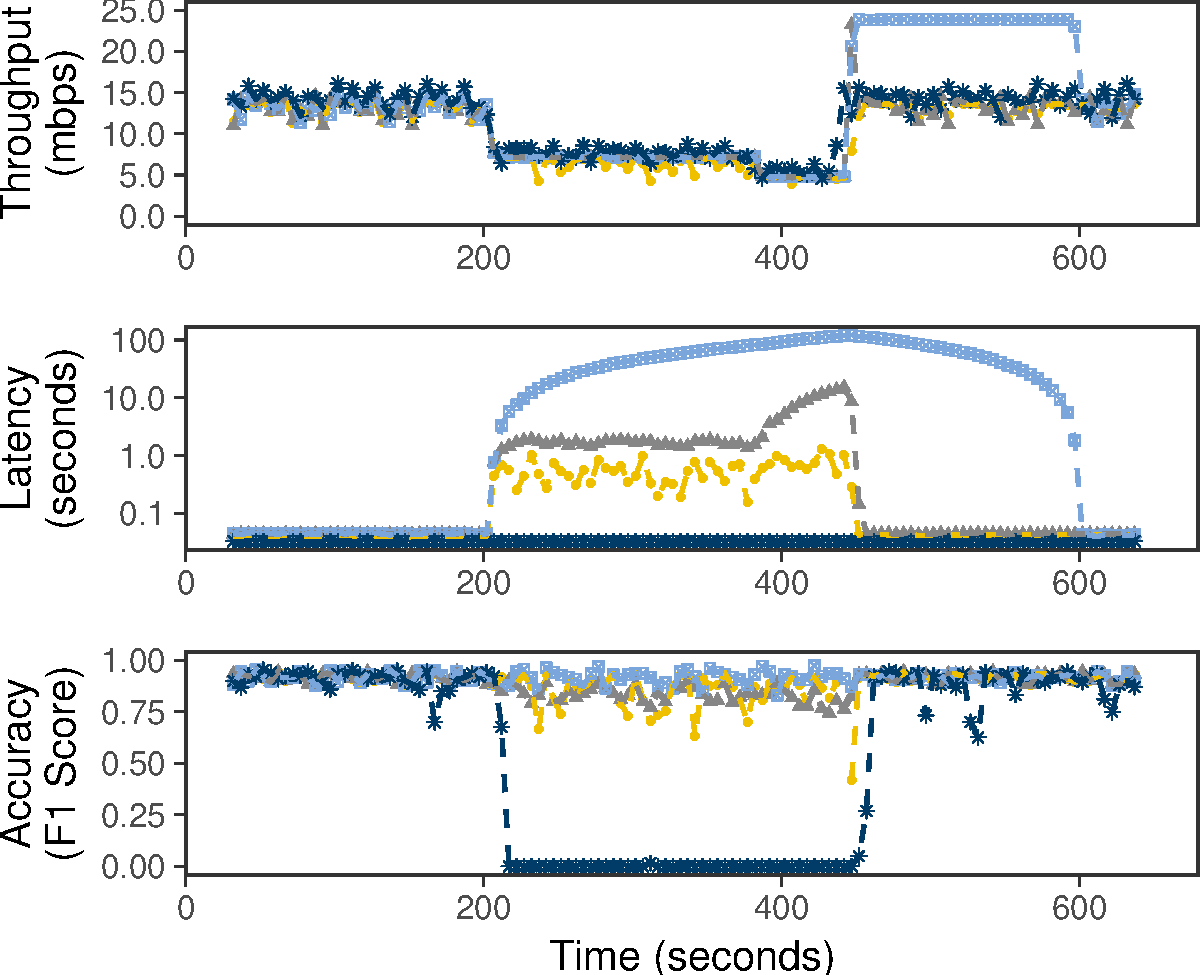
\includegraphics[width=0.8\textwidth]{figures/runtime-timeseries-3.pdf}
    \end{figure}
  }
  \only<4>{
    \begin{figure}
      \centering
      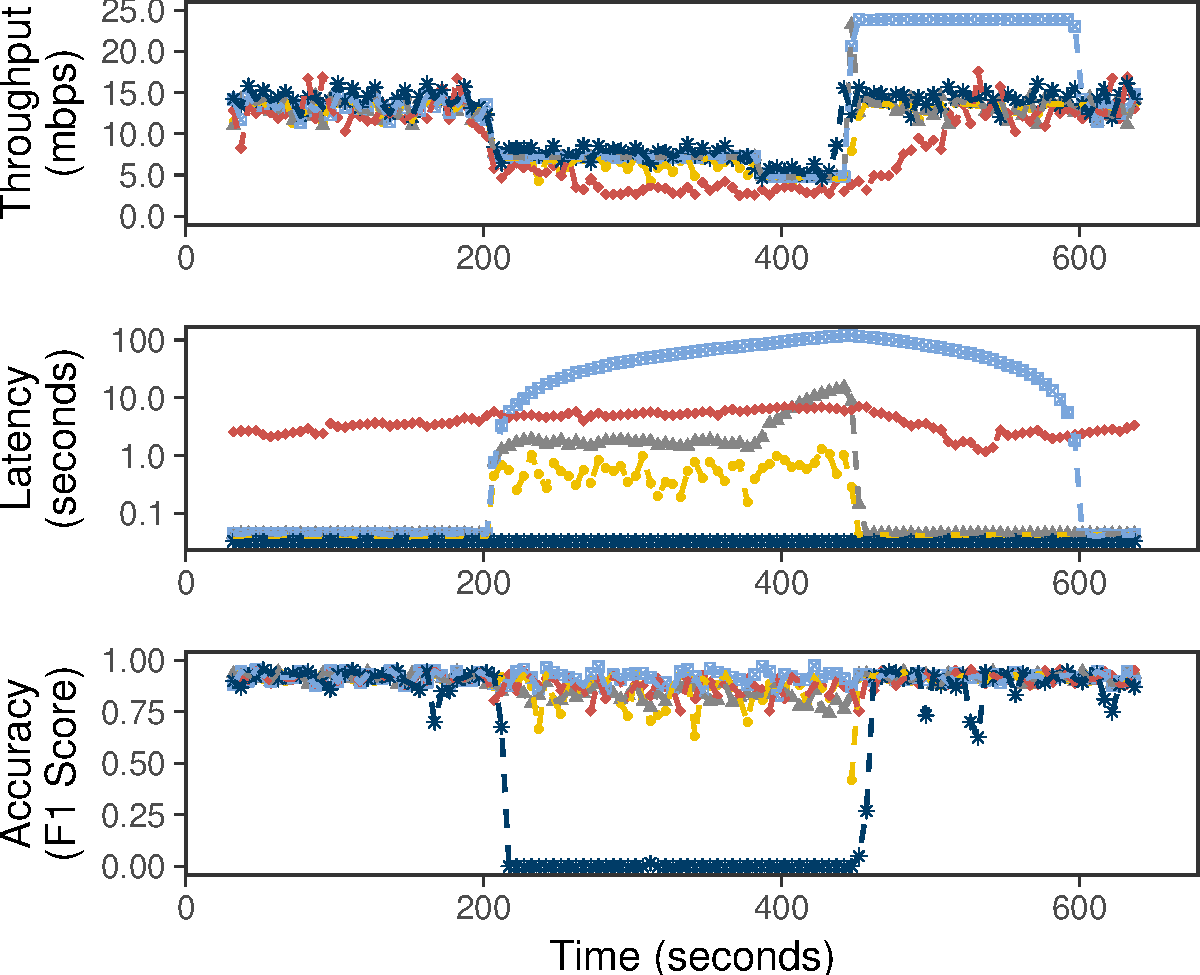
\includegraphics[width=0.8\textwidth]{figures/runtime-timeseries-4.pdf}
    \end{figure}
  }
  \only<5>{
    \begin{figure}
      \centering
      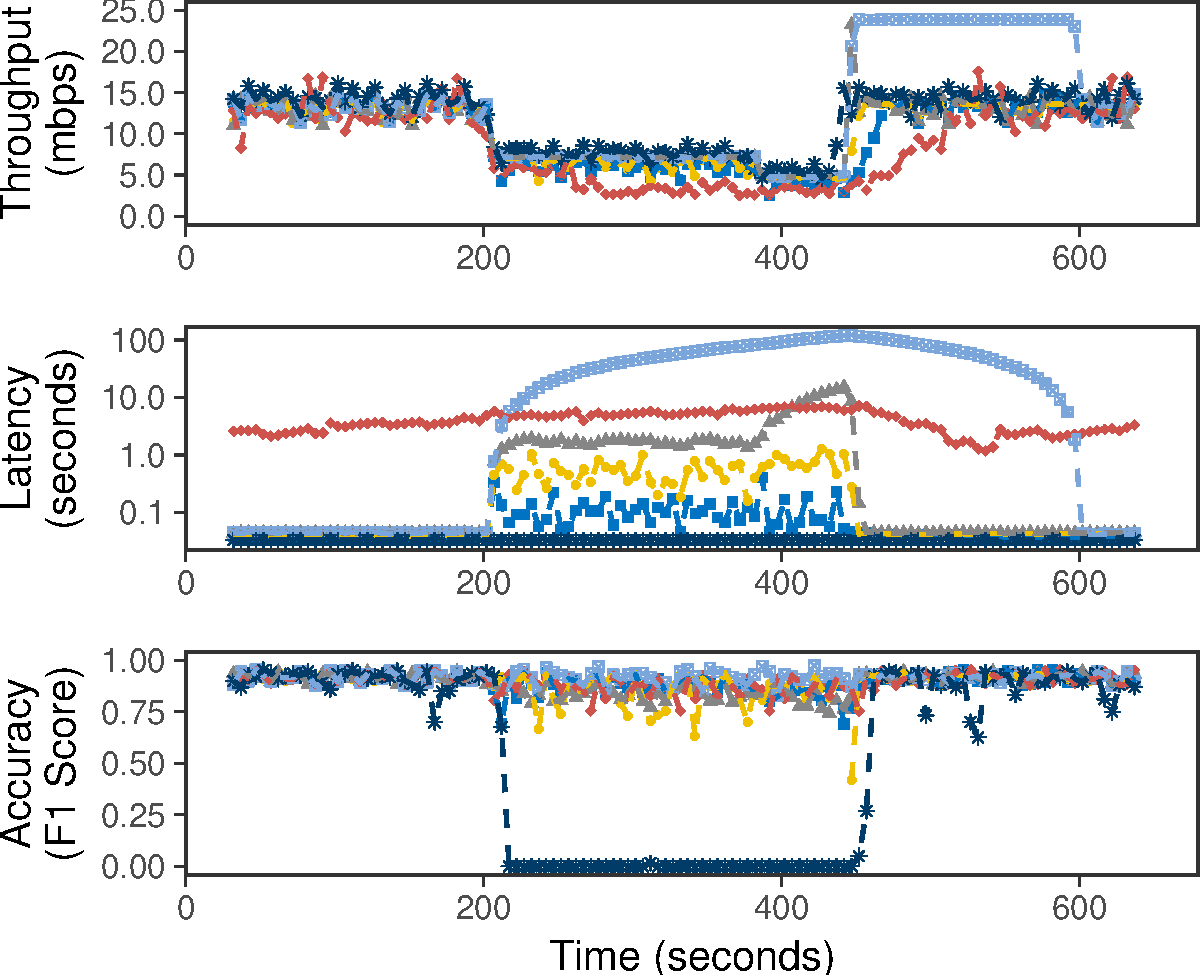
\includegraphics[width=0.8\textwidth]{figures/runtime-timeseries-5.pdf}
    \end{figure}
  }

  \only<6->{
    \begin{figure}
      \centering
      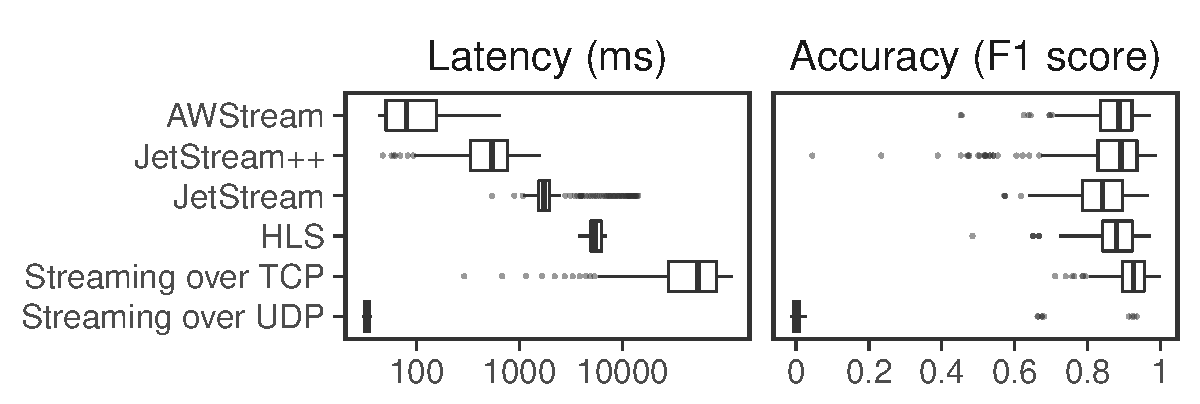
\includegraphics[width=0.8\textwidth]{figures/runtime-boxplot.pdf} \\
      \vspace{1em}
      \visible<7>{
        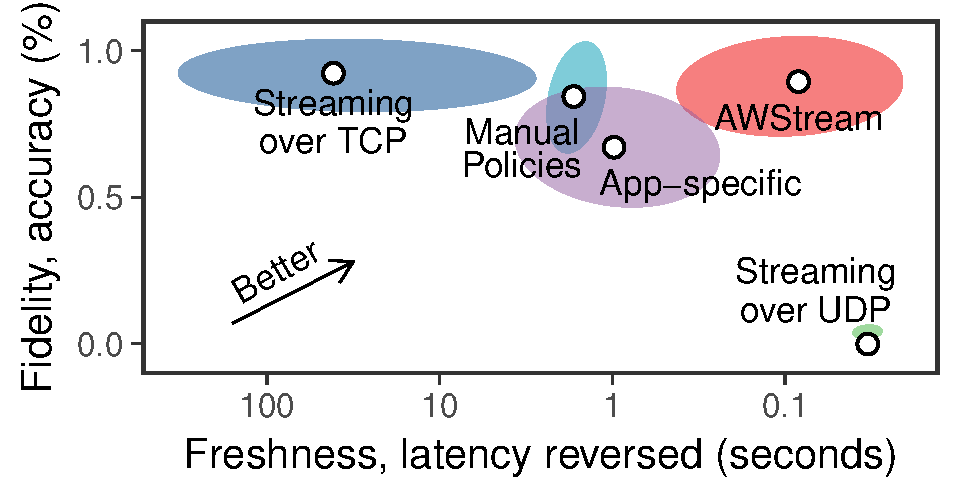
\includegraphics[width=0.6\columnwidth]{figures/fidelity-freshness-full.pdf}
      }
    \end{figure}
  }
\end{frame}

%%% Local Variables:
%%% mode: latex
%%% TeX-master: "../talk"
%%% TeX-engine: xetex
%%% End:
